\usetikzlibrary{positioning, calc, fit}

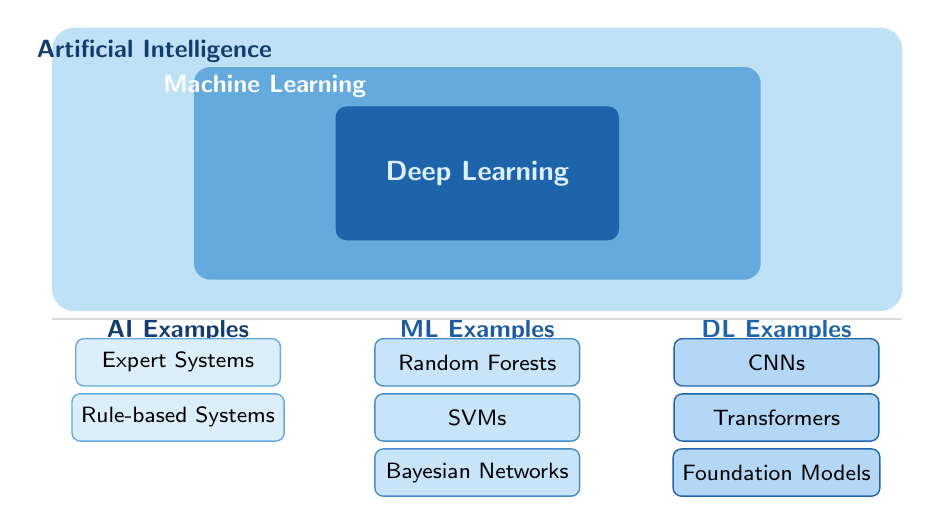
\begin{tikzpicture}[
    every node/.style={font=\small\sffamily},
    exbox/.style={
        rectangle, rounded corners=3pt,
        fill=white, draw=gray!50, line width=0.5pt,
        minimum width=2.6cm, minimum height=0.6cm,
        align=center, font=\footnotesize\sffamily
    },
    colhead/.style={font=\small\sffamily\bfseries, align=center}
]

%% ── Nested rectangles ──────────────────────────────────────────────
%% Outermost: Artificial Intelligence (light blue)
\fill[rounded corners=8pt,
      fill={rgb,255:red,190;green,225;blue,245}]
    (-5.4, 2.6) rectangle (5.4, -1.0);

%% Middle: Machine Learning (medium blue)
\fill[rounded corners=6pt,
      fill={rgb,255:red,100;green,170;blue,220}]
    (-3.6, 2.1) rectangle (3.6, -0.6);

%% Innermost: Deep Learning (dark blue)
\fill[rounded corners=4pt,
      fill={rgb,255:red,30;green,100;blue,170}]
    (-1.8, 1.6) rectangle (1.8, -0.1);

%% Labels inside each region
\node[text={rgb,255:red,220;green,240;blue,255},
      font=\normalsize\sffamily\bfseries]
    at (0, 0.75) {Deep Learning};

\node[text=white, font=\small\sffamily\bfseries]
    at (-2.7, 1.85) {Machine Learning};

\node[text={rgb,255:red,20;green,60;blue,110},
      font=\small\sffamily\bfseries]
    at (-4.1, 2.3) {Artificial Intelligence};

%% ── Example columns below ──────────────────────────────────────────
\def\rowA{-1.65}
\def\rowB{-2.35}
\def\rowC{-3.05}

%% Column headers
\node[colhead, text={rgb,255:red,20;green,60;blue,110}]
    at (-3.8, -1.25) {AI Examples};
\node[colhead, text={rgb,255:red,30;green,90;blue,160}]
    at (0,    -1.25) {ML Examples};
\node[colhead, text={rgb,255:red,30;green,100;blue,170}]
    at (3.8,  -1.25) {DL Examples};

%% AI column
\node[exbox, fill={rgb,255:red,220;green,238;blue,250},
      draw={rgb,255:red,100;green,170;blue,220}]
    at (-3.8, \rowA) {Expert Systems};
\node[exbox, fill={rgb,255:red,220;green,238;blue,250},
      draw={rgb,255:red,100;green,170;blue,220}]
    at (-3.8, \rowB) {Rule-based Systems};

%% ML column
\node[exbox, fill={rgb,255:red,200;green,228;blue,248},
      draw={rgb,255:red,70;green,140;blue,200}]
    at (0, \rowA) {Random Forests};
\node[exbox, fill={rgb,255:red,200;green,228;blue,248},
      draw={rgb,255:red,70;green,140;blue,200}]
    at (0, \rowB) {SVMs};
\node[exbox, fill={rgb,255:red,200;green,228;blue,248},
      draw={rgb,255:red,70;green,140;blue,200}]
    at (0, \rowC) {Bayesian Networks};

%% DL column
\node[exbox, fill={rgb,255:red,180;green,215;blue,245},
      draw={rgb,255:red,30;green,100;blue,170}]
    at (3.8, \rowA) {CNNs};
\node[exbox, fill={rgb,255:red,180;green,215;blue,245},
      draw={rgb,255:red,30;green,100;blue,170}]
    at (3.8, \rowB) {Transformers};
\node[exbox, fill={rgb,255:red,180;green,215;blue,245},
      draw={rgb,255:red,30;green,100;blue,170}]
    at (3.8, \rowC) {Foundation Models};

%% Thin separator line
\draw[gray!30, line width=0.4pt]
    (-5.4, -1.1) -- (5.4, -1.1);

\end{tikzpicture}
